Há quase setenta anos, após o lançamento do Sputnik-1 \citep{nasa1957} e do início de uma série de satélites com massas da ordem de toneladas \citep{sputnik3}, a União das Repúblicas Socialistas Soviéticas (URSS) demonstrou possuir foguetes com maior capacidade de carga que seus equivalentes no restante do globo. Tal feito foi fruto de um programa com alto nível de desenvolvimento, fundamentado em uma eficiente rede de pesquisa e inovação na área espacial. Esse avanço sugeria que o próximo passo natural seria a conquista da Lua e dos demais planetas do Sistema Solar \citep{betzler2024}.

Porém, menos de dez anos depois, os programas espaciais soviético e estadunidense estavam em níveis completamente diferentes. Enquanto o cosmonauta Komarov havia morrido no primeiro teste de voo da Soyuz-1 \citep{zak2018}, a missão Apollo-8 realizava com sucesso a primeira circunavegação tripulada Terra-Lua \citep{nasaApollo8}. Em julho de 1969, o primeiro pouso lunar tripulado americano foi realizado \citep{nasaApollo11}, consolidando o avanço tecnológico e estratégico dos Estados Unidos. Em contrapartida, autoridades soviéticas anunciaram oficialmente que nunca houve um programa destinado ao pouso de cosmonautas na superfície lunar \citep{betzler2024}.

Com o fim da URSS, em 1991, documentos secretos começaram a ser liberados, revelando informações que contradiziam as declarações oficiais. As razões para a falta de êxito da URSS em colocar cosmonautas na superfície lunar são complexas e variadas, abrangendo desde limitações técnicas e políticas até questões estratégicas \citep{betzler2024}. A utilização dos foguetes como ferramenta estratégica ganhou impulso significativo na União Soviética após a Segunda Guerra Mundial, com a percepção de que essa tecnologia poderia definir o equilíbrio de poder global. Durante esse período, a pesquisa soviética esteve concentrada no desenvolvimento de tecnologias de foguetes voltadas para aplicações militares, como sistemas de decolagem assistida (JATO) \citep{glushko1973} e aeronaves movidas a motores-foguete. Projetos como o RP-318 \citep{RP318}, o BI-1 \citep{BI1} e o Malyutka \citep{Malyutka} foram exemplos iniciais desse esforço, mas o grande avanço veio com a captura e estudo das tecnologias alemãs após a guerra, especialmente os foguetes V-2.

Foi nesse contexto que o trabalho relativo aos foguetes de grande alcance começou a tomar forma, com projetos como o Tikhonravov MK e os mísseis D-1 e D-2 liderando o caminho. No entanto, as limitações de infraestrutura, recursos e conhecimento interno tornaram evidente a necessidade de uma abordagem mais organizada e estratégica. Em resposta, a URSS iniciou em 1946 o desenvolvimento de mísseis de longo alcance \citep{siddiqi2004}, um decreto que estabelecia institutos de pesquisa especializados no desenvolvimento de foguetes, com a transferência de milhares de técnicos alemães para colaborar nesses esforços. Esses institutos rapidamente se tornaram centros de inovação tecnológica, liderados por nomes como Mstislav Keldysh e Aleksei Isayev, que supervisionaram projetos como o Bombardeiro Keldysh e os mísseis intercontinentais Buran e Burya. Apesar dos avanços significativos, o programa espacial soviético enfrentava desafios estruturais, como a fragmentação de esforços entre diferentes projetistas e disputas internas por liderança. Contudo, o desenvolvimento dessas tecnologias estabeleceu a base para os marcos posteriores do programa espacial soviético, incluindo o lançamento do Sputnik-1 em 1957, que marcou o início da era espacial e consolidou a URSS como uma potência tecnológica global \citep{betzler2024}.

A partir de 1956, o programa espacial soviético avançou com planos concretos e objetivos ambiciosos. O governo soviético definiu três metas principais \citep{betzler2024}: (I) lançar satélites artificiais com massa entre 1,80 e 2,50 toneladas até 1958, (II) desenvolver um satélite de reconhecimento não tripulado até 1970 e (III) realizar voos espaciais tripulados com duração de até uma semana até 1964. Esses objetivos eram parte de uma estratégia abrangente para consolidar a liderança soviética na exploração espacial, equilibrando as prioridades militares e científicas. A primeira meta, associada ao lançamento do satélite artificial terrestre (ISZ), foi iniciada com estudos em laboratório sobre o meio ambiente espacial. Em julho de 1956, o desenvolvimento do ISZ foi concluído, e a construção do satélite e seus sistemas de acompanhamento terrestre foi autorizada por um decreto em setembro do mesmo ano. No entanto, devido à pressão de lançar um satélite antes dos americanos, o projeto ISZ foi temporariamente adiado, e dois pequenos satélites, Sputnik-1 e 2, foram rapidamente construídos para cumprir essa meta \citep{betzler2024}.

O lançamento do Sputnik-1 em 4 de outubro de 1957 \citep{nasaSputnik1} marcou o início da era espacial, tornando-se o primeiro satélite artificial a orbitar a Terra. Essa realização colocou a União Soviética à frente na corrida espacial, mas foi também uma demonstração de força militar e tecnológica em plena Guerra Fria. Com uma esfera de alumínio de 58 cm de diâmetro e 83,60 kg, o Sputnik-1 destacou o pioneirismo soviético na Astronáutica. Pouco depois, o Sputnik-2 foi lançado, levando a bordo a cadela Laika \citep{nasaSputnik2} , o primeiro ser vivo a orbitar a Terra. Embora essas conquistas representassem avanços científicos, também eram fruto de disputas internas entre militares e civis sobre as prioridades do programa espacial. Enquanto os militares priorizavam satélites de reconhecimento, os civis, liderados por Korolev, advogavam pela importância de missões tripuladas \citep{betzler2024}.

Em 1958, o projeto Vostok \citep{nasaVostok1} começou a ganhar forma, associado ao objetivo de realizar voos tripulados. Inicialmente, o trabalho ocorreu em paralelo ao projeto militar Zenit, que visava o desenvolvimento de satélites de reconhecimento fotográfico. Korolev defendeu que a tecnologia do Zenit \citep{astronautixZenit} poderia ser utilizada como base para os voos tripulados, o que resultou na unificação parcial dos esforços. O primeiro voo tripulado da Vostok ocorreu em 12 de abril de 1961, com Yuri Gagarin tornando-se o primeiro ser humano a orbitar a Terra. A missão foi um marco na história da exploração espacial, quebrando recordes de velocidade e altitude para um veículo tripulado. No entanto, a missão enfrentou desafios significativos, incluindo falhas durante a reentrada, que exigiram que Gagarin ejetasse da cápsula antes do pouso. Apesar disso, o sucesso da missão consolidou a posição soviética como líder na corrida espacial \citep{betzler2024}.

O programa Vostok foi seguido por novas iniciativas destinadas a expandir as capacidades soviéticas no espaço. As missões subsequentes buscavam não apenas avançar tecnologicamente, mas também reforçar o prestígio internacional da URSS. No entanto, os desafios estruturais do programa, como disputas entre projetistas, fragmentação de esforços e limitações de financiamento, começaram a impactar negativamente os avanços. Além disso, os Estados Unidos intensificaram seus esforços com o programa Apollo, superando a URSS na corrida para o pouso lunar. Apesar dessas dificuldades, o legado do programa espacial soviético permanece como uma das mais impressionantes realizações tecnológicas do século XX, destacando a capacidade de inovação em um contexto de recursos limitados e intensas pressões políticas \citep{betzler2024}.

\subsection{Estação espacial Skylab (EUA)}

Skylab, a primeira estação espacial americana, representou um marco na exploração espacial dos Estados Unidos, consolidando o avanço tecnológico do país após a corrida espacial contra a União Soviética. Desenvolvido a partir da terceira fase do programa Apollo, o Skylab foi projetado para utilizar os conhecimentos e tecnologias adquiridos durante as missões lunares, adaptando-os para objetivos científicos e de longo prazo em órbita terrestre. Lançado em 14 de maio de 1973, o Skylab tinha como missão principal realizar experimentos científicos em microgravidade, estudar a Terra e o Sol, além de compreender os efeitos do ambiente espacial em seres humanos durante estadias prolongadas \citep{nasaSkylab}.

\begin{figure}[H]
    \centering
    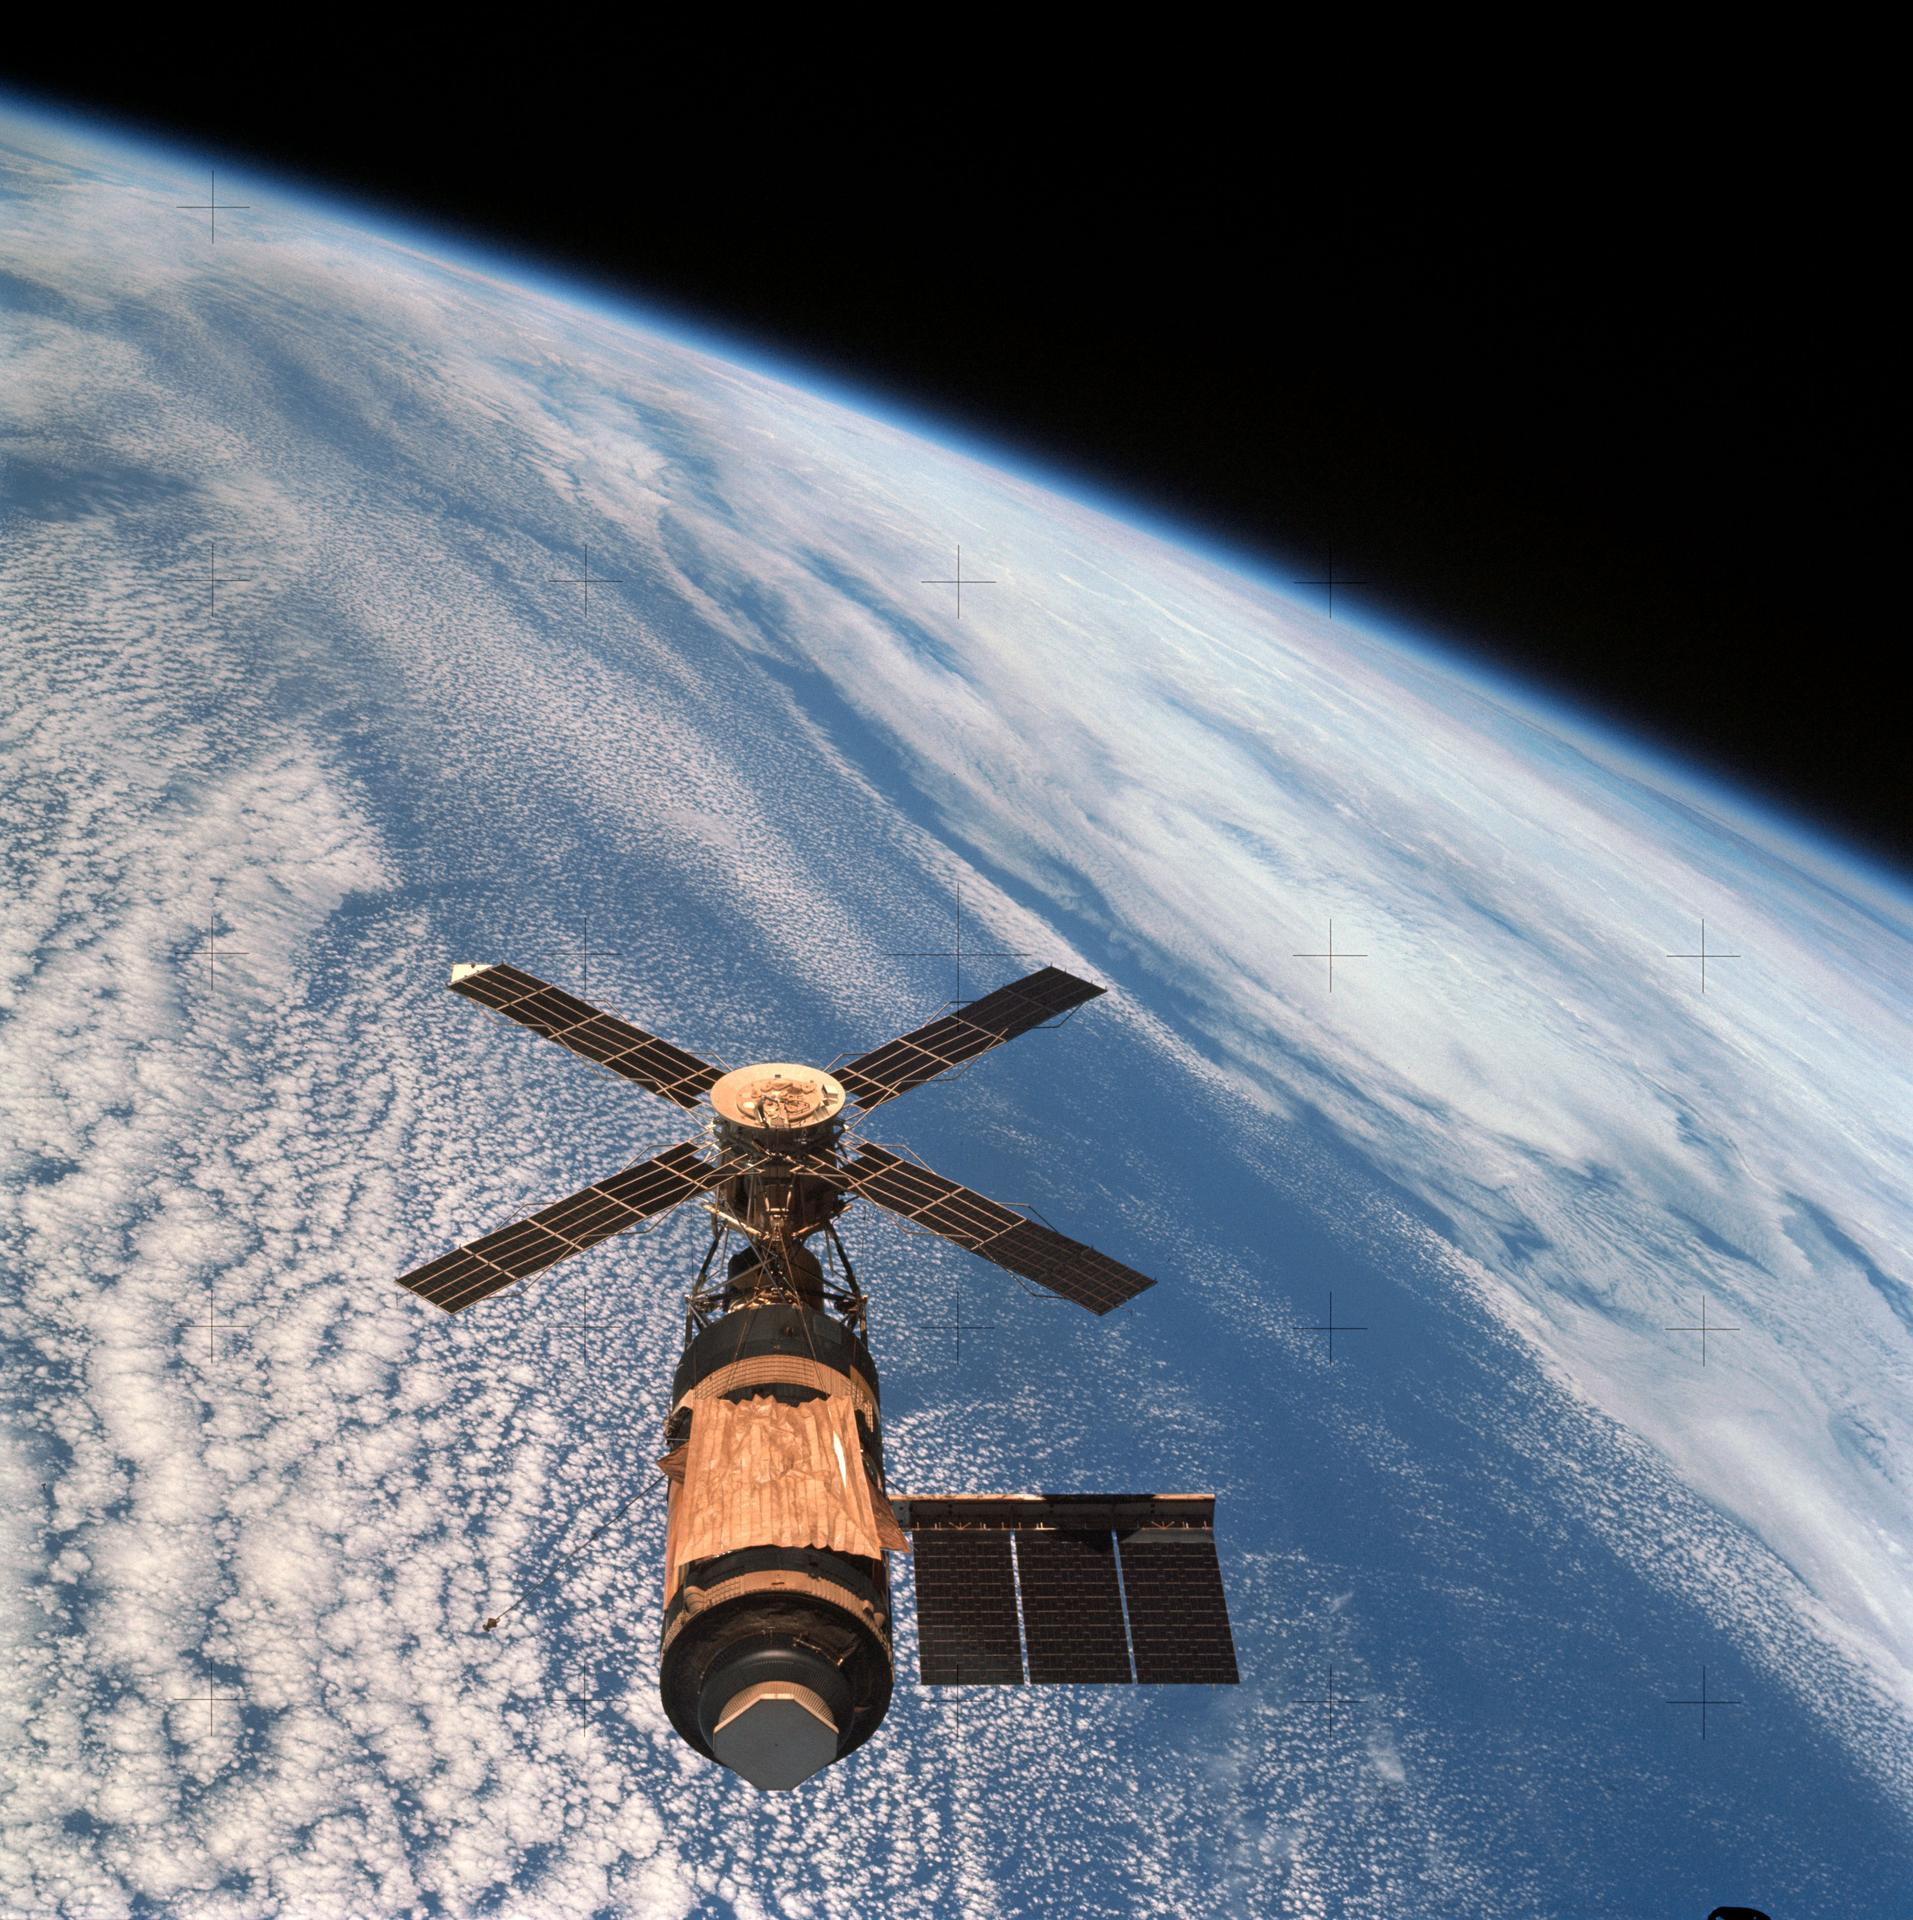
\includegraphics[width=0.75\linewidth]{Imagens/Skylab NASA.jpg}
    \caption{A Estação Espacial Skylab orbitando a Terra. Fonte: Nasa \\ (\url{https://www.nasa.gov/gallery/skylab}).}
    \label{fig:SkylabFoto}
\end{figure}

A estrutura do Skylab era baseada no segundo estágio de um foguete Saturno V modificado, transformado em um laboratório espacial. Essa abordagem permitiu economizar custos e aproveitar a infraestrutura existente. O Skylab era dividido em módulos, incluindo o laboratório orbital, o módulo de múltiplos usos, a estação de controle e o módulo solar, além disso, a estação contava com painéis solares que forneciam energia para os experimentos e para a manutenção do ambiente interno. Os avanços tecnológicos implementados no Skylab permitiram que a tripulação realizasse experimentos complexos, incluindo observações solares com o uso de telescópios especializados, estudos de ciências da vida e experimentos em física de fluidos \citep{nasaSkylab}.

As missões tripuladas para o Skylab foram realizadas por meio de naves Apollo modificadas, que transportaram astronautas para estadias de longa duração na estação. Três tripulações visitaram o Skylab entre 1973 e 1974, cada uma estabelecendo recordes crescentes de permanência em órbita. Durante essas missões, os astronautas realizaram muitos experimentos científicos e contribuíram significativamente para o conhecimento sobre os efeitos da microgravidade \citep{nasaSkylab}.

Apesar de seu sucesso científico, o Skylab enfrentou desafios operacionais desde o início. Durante o lançamento, a estação sofreu danos significativos, incluindo a perda de um escudo térmico e um dos seus principais painéis solares \citep{nasaSkylab2}. Esses problemas comprometeram a capacidade da estação de gerar energia e regular sua temperatura interna. No entanto, com o apoio de engenheiros em terra e a habilidade da primeira tripulação, reparos improvisados foram realizados, incluindo a instalação de um escudo solar para reduzir a temperatura interna e a liberação manual de um painel solar preso. Essas operações destacaram a capacidade de inovação e adaptação da NASA em situações de crise \citep{nasaSkylab}.

Embora o Skylab tenha superado muitos dos seus desafios iniciais, a estação não estava preparada para resistir indefinidamente em órbita. Em 1979, após anos de abandono devido à falta de capacidade da NASA para realizar missões de manutenção com o Space Shuttle, o Skylab reentrou na atmosfera terrestre, com partes de seus destroços caindo na Austrália Ocidental \citep{nasaSkylabReentry}. Apesar de seu fim abrupto, o legado do Skylab permanece significativo. Ele serviu como uma plataforma de aprendizado crucial para o desenvolvimento de estações espaciais modernas, estabelecendo os alicerces para programas como o da ISS. Além disso, as descobertas científicas realizadas no Skylab continuam a influenciar a compreensão de questões fundamentais sobre a vida e o trabalho no espaço \citep{nasaSkylab}.

O Skylab demonstrou que uma estação espacial pode ser um ambiente de pesquisa multifuncional, capaz de integrar estudos em várias disciplinas científicas enquanto oferece suporte à vida humana em condições extremas. Ele marcou uma transição importante na exploração espacial, mostrando que os esforços humanos no espaço podem ir além das missões lunares e abrir novos caminhos para a ciência e a tecnologia. Com isso, o Skylab consolidou seu papel como um marco histórico na era da exploração espacial americana \citep{nasaSkylab}.

\subsection{Acoplamento automático entre duas espaçonaves}

O problema de realizar o acoplamento automático de duas espaçonaves tem sido historicamente negligenciado devido à disponibilidade de pilotos humanos que assumiam essa função. Contudo, a União Soviética demonstrou um sistema para acoplamento automático entre dois veículos controlados e ativos, destacando a necessidade de explorar sistemas mais avançados. Durante o período em que o estudo foi conduzido, em 1981, ainda não havia sido amplamente desenvolvido ou testado em voo um esquema automático de acoplamento em que um dos veículos permanecesse completamente inativo. Essa lacuna tecnológica, identificada naquela época, evidenciava a necessidade de avançar na capacidade de acoplamento automático, especialmente para aplicações como a recuperação de satélites e a construção de estruturas espaciais \citep{micheal1981}.

O trabalho apresentado por \citep{micheal1981} surgiu como parte do projeto Teleoperator Retrieval System (TRS), cuja missão inicial era impulsionar o Skylab para uma órbita mais alta, prolongando sua vida útil no espaço. Durante o desenvolvimento do TRS, simulações híbridas de seis graus de liberdade, envolvendo operadores humanos no ciclo de controle, foram realizadas para analisar os problemas associados ao acoplamento entre o TRS e o Skylab. Essas simulações destacaram os desafios técnicos enfrentados por astronautas experientes e motivaram a investigação de sistemas de acoplamento autônomo.

O estudo abordou um cenário de missão representativo para identificar os requisitos de extração de dados de atitude e posição relativa. Um sistema de acoplamento autônomo foi simulado digitalmente, utilizando dispositivos como sensores de varredura a laser e câmeras de vídeo. Os resultados dessas simulações demonstraram que o desenvolvimento de esquemas automáticos de acoplamento baseados em vídeo poderia representar um avanço significativo em operações de acoplamento em órbita. Além disso, o trabalho enfatizou a necessidade de maior integração entre sistemas de sensoriamento e algoritmos de controle para reduzir o tempo de treinamento e aumentar a eficiência operacional \citep{micheal1981}.

As investigações realizadas no estudo de \citep{micheal1981} não apenas destacaram os desafios do acoplamento autônomo, mas também forneceram visões valiosas para o desenvolvimento de tecnologias mais avançadas. Esse esforço inicial foi fundamental para a evolução de sistemas de acoplamento automáticos modernos, que hoje desempenham um papel essencial em missões como a ISS. A transição de sistemas manuais para automáticos, conforme discutido no trabalho, marcou um avanço importante na capacidade de realizar operações espaciais complexas com maior autonomia e confiabilidade \citep{micheal1981}.

\subsection{Colaboração internacional}

A Estação Espacial Internacional (ISS) é uma das maiores realizações da cooperação internacional na exploração espacial. Desde sua montagem em 1998, a ISS tem servido como um laboratório de microgravidade e um centro de pesquisa científica em órbita terrestre. Ela foi desenvolvida em parceria entre cinco agências espaciais: NASA (Estados Unidos), Roscosmos (Rússia), ESA (Europa), JAXA (Japão) e CSA (Canadá), representando um marco na colaboração tecnológica global. A ISS orbita a Terra a uma altitude média de 400 quilômetros e completa aproximadamente 16 órbitas por dia, oferecendo uma plataforma única para experimentos científicos que não seriam possíveis na Terra \citep{nasaISS}.

\begin{figure}[H]
    \centering
    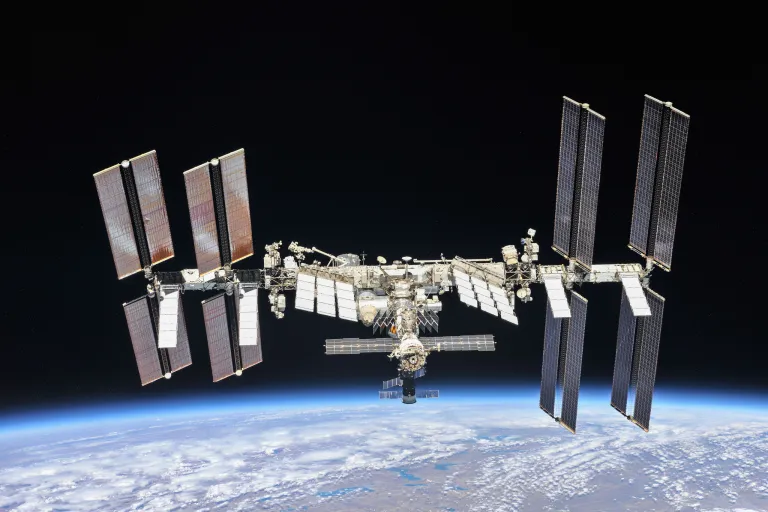
\includegraphics[width=0.75\linewidth]{Imagens/ISS NASA.png}
    \caption{A Estação Espacial Internacional (ISS) orbitando a Terra. Fonte: NASA (\url{https://www.nasa.gov/reference/international-space-station/}).}
    \label{fig:ISSfoto}
\end{figure}

A principal contribuição da ISS é no avanço da ciência em diversas áreas, incluindo biologia, física, ciência dos materiais e astronomia. Pesquisas realizadas a bordo da estação têm proporcionado visões valiosas sobre os efeitos de longo prazo da microgravidade no corpo humano, contribuindo diretamente para o planejamento de missões de exploração a longo prazo, como para Marte. Além disso, a ISS tem desempenhado um papel importante no teste de tecnologias necessárias para operações espaciais prolongadas, incluindo sistemas de suporte à vida, reciclagem de água e geração de energia solar \citep{nasaISS}.

A construção da ISS foi um empreendimento monumental, exigindo mais de 30 missões de montagem realizadas por naves espaciais como o Space Shuttle. A estação é composta por diversos módulos conectados, cada um projetado para funções específicas, como laboratórios de pesquisa, áreas de habitação e módulos de suporte técnico. O sistema de acoplamento da ISS é outro elemento importante, permitindo a chegada de veículos de carga e tripulação, como as cápsulas Dragon \citep{spacexDragon}, Cygnus \citep{northropCygnus} e Soyuz \citep{nasaSoyuz}. Essas capacidades garantem o fornecimento contínuo de suprimentos e a troca de tripulações, que geralmente permanecem em períodos de seis meses \citep{nasaISS}.

Além de suas contribuições científicas, a ISS também promove a diplomacia e a cooperação internacional. Cientistas e astronautas de diversas nações trabalham juntos para realizar pesquisas e operações diárias, criando um ambiente de colaboração global. A estação também serve como uma ferramenta educacional, inspirando novas gerações de cientistas e engenheiros por meio de programas de divulgação e parcerias com instituições educacionais \citep{nasaISS}.

À medida que a ISS se aproxima do fim de sua operação planejada, prevista para 2030 \citep{nasaISSPlan}, as agências espaciais globais estão avaliando o futuro da exploração em órbita terrestre. A estação estabeleceu as bases para futuras estações espaciais comerciais e para missões ainda mais ambiciosas no espaço profundo. O legado da ISS, portanto, vai além das suas contribuições científicas e tecnológicas, representando o potencial da humanidade de trabalhar em conjunto para objetivos comuns \citep{nasaISS}.



